\chapter{Implementation}
\thispagestyle{special}
\section{Creating Database Connection}
\begin{itemize}
\item{You can connect your deployments by either: Providing your connection string. Specifying
Advanced Connection Options. Advanced connection options allow you to specify authentication,
TLS/SSL, and SSH connection options.}
\item{Here we make use of MongoDB Compass which is a GUI for MongoDB to establish connection to
our server.}
\item{Connect to the MongoDB Server 3.1 db = connect(”localhost:27017/myDatabase”)}
\item{ Access the database
4.1.db.myNewCollection1.insertOne( x: 1 )}
\end{itemize}
\section{Architecture used(4-tier architecture)}
\centerline{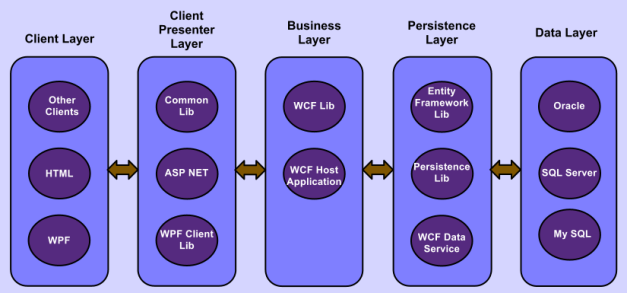
\includegraphics[scale=0.8]{N-Tier_Diagram.png}}
		\end{figure}
    Four Tier architecture is a client–server architecture in which presentation, application processing, 
and data management functions are physically separated. Four-tier application architecture 
provides a model by which developers can create flexible and reusable applications. By 
segregating an application into tiers, developers acquire the option of modifying or adding a 
specific layer, instead of reworking the entire application
\subsubsection{Presentation layer}
This is the topmost level of the application. The presentation tier displays information related to 
services such as browsing merchandise, purchasing and shopping cart contents. It also 
communicates with other tiers and puts out the results to the browser/client tier and to all other 
tiers in the network. In simple terms, it is a layer which users can access directly (such as a web 
page, or an operating system's GUI).
\subsubsection{Business Layer}
Business layer or domain logic is the part of the program that encodes the real-world business rules 
which determine how data can be created, stored, and changed. It is contrasted with the remainder 
of the software that might be concerned with lower-level details of managing a database or 
displaying the user interface, system infrastructure, or generally connecting various parts of the 
program.
\subsubsection{Data access layer}
A Data Access Layer (DAL) in computer software, is a layer of computer program which provides 
simplified access to data stored in persistent storage.
For example, the DAL might return a reference to an object (in terms of object-oriented 
programming) with its attributes instead of a row of fields from a database table. This allows the 
client (or user) modules to be created with a higher level of abstraction. This kind of model could 
be implemented by creating a class of data access methods that directly reference a corresponding 
set of database stored procedures. Another implementation could potentially retrieve or write 
records to or from a file system. The DAL hides the complexity of the underlying data store from 
the external world.
\subsubsection{Control layer}
The control layer is responsible for the communication between business and presentation layer. 
It connects logic and data with each other and provides a better connectivity and separation 
between layers
\subsection{Pseudo Code For Major Functionalities}
\textbf{Companies page:} To display Company names.\\\\
{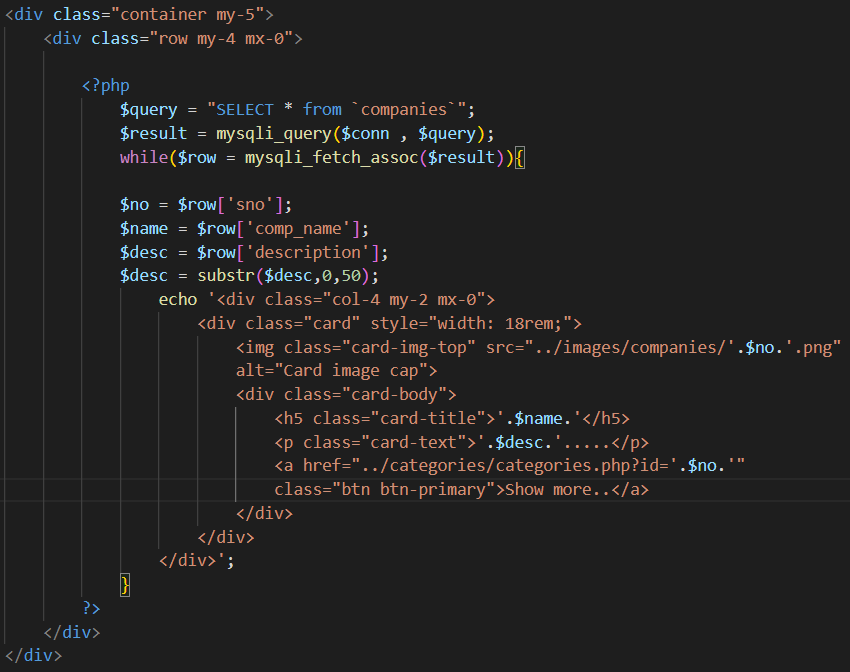
\includegraphics[scale=0.8]{image1.png}}\
		\end{figure}
Fig.3.2. Landing Page Code Snippet\\\\\\\\\\\\\\\\\\\\\\\\\\
\textbf{List page:} To list the data present for a particular company.\\\\
{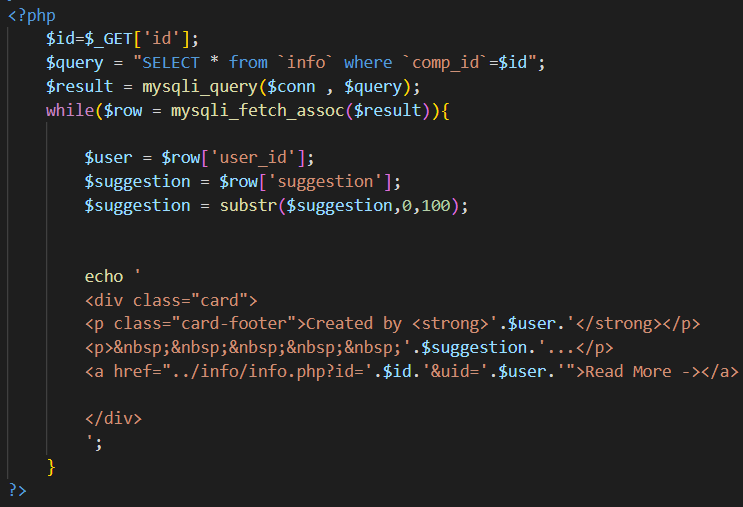
\includegraphics[scale=0.9]{image2.png}}\
		\end{figure}
    Fig.3.3. List Page Code Snippet  \\\\\\\\\\\\\\\\\\\\\\\\\\\\\\

\textbf{Data page:} To Represent a data inserted by a particular user.\\\\
{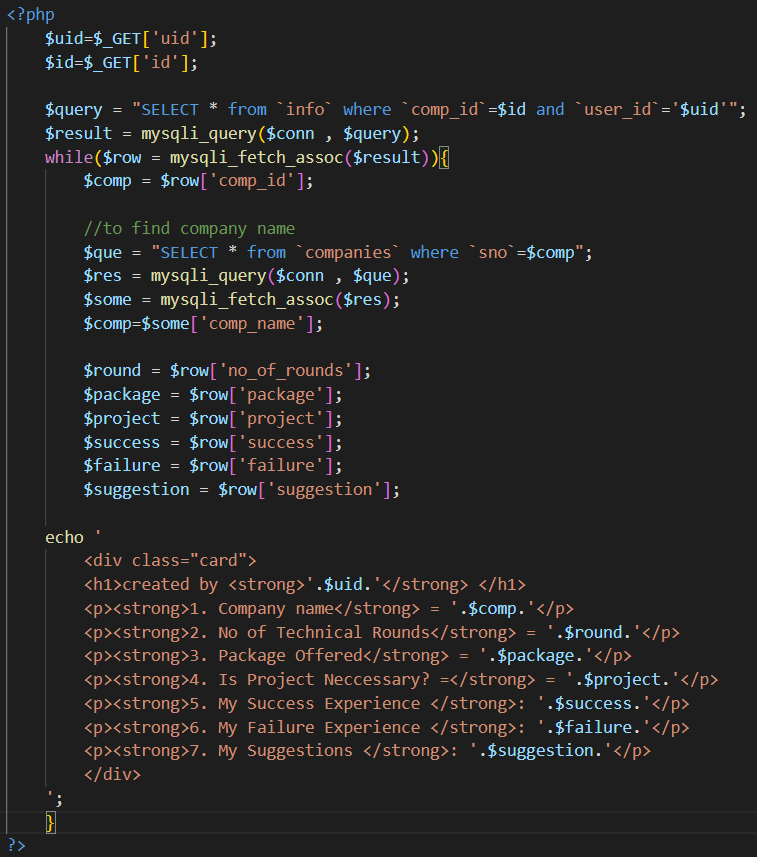
\includegraphics[scale=0.9]{image3.png}}\
		\end{figure}
    Fig.3.4. Data Page Code Snippet  